\section{FieldFormer}
\label{sec:method}
\subsection{Design Rationale}
FieldFormer is designed around three core principles motivated by sparse, longitudinal spatio-temporal data:

\begin{itemize}[leftmargin=*,topsep=0pt]
    \item \textbf{Local--Global Information Mixing:}
    Prior work by \cite{bhardwaj2025comprehensive}has shown that purely local methods (e.g., Kriging) are effective under sparse sensing, while global neural fields can capture long-range dependencies but struggle in longitudinal regimes. FieldFormer combines local neighborhood encoding with global coordinate information using transformer-based attention, enabling relational reasoning across space and time while retaining strong local inductive bias. Although attention is restricted to local neighborhoods, predictions remain globally grounded through continuous coordinates.

    \item \textbf{Learned Neighborhood Geometry:}
    Global attention incurs $O(n^2)$ memory cost, which is prohibitive for temporally dense sensing. FieldFormer instead performs attention over compact local neighborhoods, whose geometry is learned from data and physics priors. This allows the model to attend selectively to physically relevant regions while remaining memory-efficient and scalable.

    \item \textbf{Mesh-Free Modeling:}
    FieldFormer adopts a mesh-free coordinate-based representation along with a local spatio-temporal context, enabling inference at arbitrary spatial and temporal resolutions. This makes the model naturally adaptable to evolving sensor networks. For example, when a new sensor is deployed, its measurements can be incorporated as additional coordinate-value observations without redefining the spatial grid, rebuilding a graph adjacency matrix, or changing the model architecture. Similarly, if sensors fail, move, or are added in previously unobserved regions, the model can continue operating by constructing neighborhoods from the updated set of available observations.
\end{itemize}


\subsection{Architecture}
\begin{figure*}
    \centering
    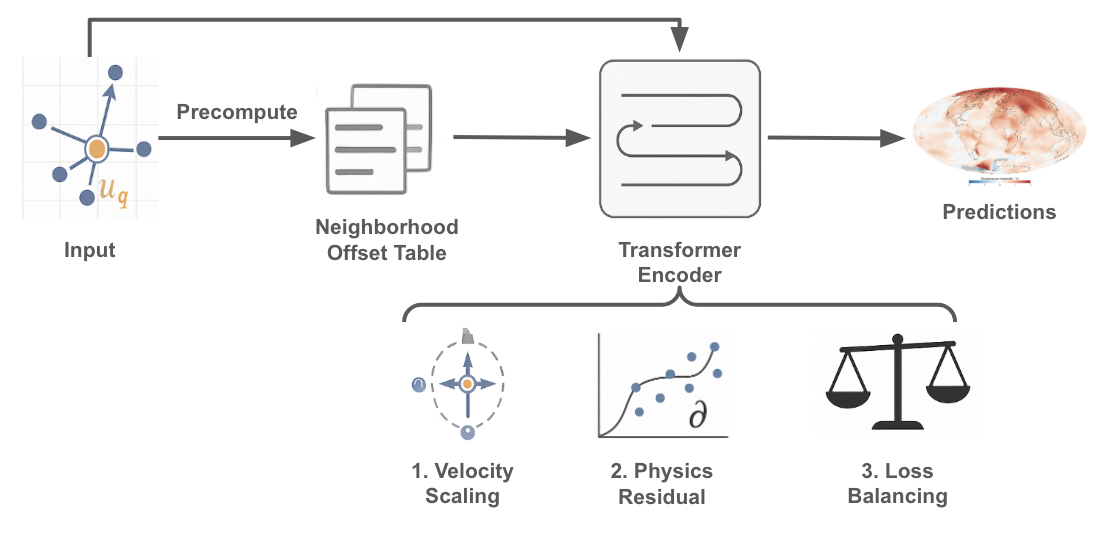
\includegraphics[width=0.95\linewidth]{concept.png}
    \caption{\small Conceptual overview of FieldFormer. For each query location, a physics-aware local neighborhood is constructed via learned velocity scaling, encoded with relative offsets and observations, and aggregated using a transformer encoder to produce mesh-free spatio-temporal predictions, trained with data and optionally balanced physics losses.}
    \label{fig:concept}
\end{figure*}

\noindent\textbf{Local Neighborhood Encoding:}  
Predicting the field value at a query $(\mathbf{x}_q, t_q) \in \mathbb{R}^{d_s} \times \mathbb{R}$ requires local context: PDEs, especially with \textit{local operators}, typically couple a state variable to its spatial and temporal neighbors rather than to the entire domain. To emulate this, FieldFormer extracts a fixed-size local neighborhood from the dataset
\[
\mathcal{D} = \{ (\mathbf{x}_i, t_i, \mathbf{u}_i) \}_{i=1}^N, \quad \mathbf{u}_i \in \mathbb{R}^q.
\]

Neighbors are not chosen by naive Euclidean distance, but by a \emph{velocity-scaled metric} that adapts to anisotropic dynamics:
\begin{equation}
\label{eq:velocity_distance}
d\big( (\mathbf{x}_q, t_q), (\mathbf{x}_i, t_i) \big) 
= \sum_{k=1}^{d_s} \gamma_k^2 (x_{q,k} - x_{i,k})^2 + \gamma_t^2 (t_q - t_i)^2.
\end{equation}
The learnable parameters $\{\gamma_k\}_{k=1}^{d_s}, \gamma_t$ weight each spatial axis and time relative to one another. They are parameterized as $\gamma = \exp(\theta)$ to enforce positivity. This scaling allows the model to \emph{discover} the anisotropy of the underlying process: for purely diffusive systems it may amplify temporal proximity, while for advective or wave-like systems it stretches neighborhoods preferentially along flow directions. Thus the model automatically learns whether a time step is "worth" more than a spatial offset.

Each neighbor $(\mathbf{x}_j, t_j, \mathbf{u}_j)$ is encoded relative to the query:
\[
\mathbf{v}_j = \big[\, \mathbf{x}_j - \mathbf{x}_q,\;\; t_j - t_q,\;\; \mathbf{u}_j \,\big] \in \mathbb{R}^{d_s+1+q},
\]
resulting in an input matrix $\mathbf{X}_q \in \mathbb{R}^{n \times (d_s+1+q)}$. This encoding is translation-invariant and emphasizes relative differences, which is crucial when queries are at unseen coordinates.

\noindent\textbf{Sparse Neighborhood Construction.}
A practical challenge in sparse longitudinal sensing is that the model must construct a local spatio-temporal context from incomplete observations without relying on a dense grid or repeatedly performing query-wise nearest-neighbor search. FieldFormer handles this by operating directly on observed sensor-time tuples. Each available observation is represented as $(\mathbf{x}_s,t_k,\mathbf{u}_{s,k})$, indexed by sensor location $s$ and time index $k$. For a query $(\mathbf{x}_q,t_q)$, FieldFormer constructs a fixed maximal longitudinal context
\[
\mathcal{C}(q)
=
\mathcal{S}_K(q)
\times
\{t_q-K_t,\ldots,t_q+K_t\},
\]
where $\mathcal{S}_K(q)$ denotes a small spatial candidate set of nearby sensor locations and $K_t$ is the temporal window radius. Missing observations are excluded from this context, and the remaining valid observations are padded or truncated to produce a fixed-size set of $K$ tokens for transformer aggregation.

This fixed-context construction is a differentiable and efficient relaxation of learned metric-based neighbor selection. Given a query $q$, the learned spatio-temporal metric can be written as
\[
d_q(i)
=
\gamma_x(q)^2 \Delta x_i^2
+
\gamma_y(q)^2 \Delta y_i^2
+
\gamma_t(q)^2 \Delta t_i^2 ,
\]
where $\Delta x_i=x_i-x_q$, $\Delta y_i=y_i-y_q$, and $\Delta t_i=t_i-t_q$. Once the relevant spatial candidates are included in $\mathcal{S}_K(q)$, the temporal component of the metric is monotone in $|\Delta t_i|$. Therefore, for a sufficiently large temporal window, the fixed context contains the metric-$k$NN neighborhood as a subset:
\[
\mathrm{kNN}_{d_q}(q) \subseteq \mathcal{C}(q).
\]
Rather than selecting a hard metric-dependent subset whose membership changes discontinuously as $\gamma$ evolves, FieldFormer includes this local superset and lets the model learn relevance through metric-conditioned token features.

Concretely, for each candidate observation, FieldFormer computes relative offsets and scales them by positive learned factors,
\[
(\widetilde{\Delta x}_i,\widetilde{\Delta y}_i,\widetilde{\Delta t}_i)
=
(\gamma_x \Delta x_i,\gamma_y \Delta y_i,\gamma_t \Delta t_i),
\qquad
\gamma=\exp(\theta),
\]
with periodic wrapping for spatial coordinates when appropriate. These scaled offsets are concatenated with the observed value to form each input token. Thus, the learned geometry does not determine hard inclusion in the neighborhood; instead, it controls how the transformer interprets spatial and temporal separation within a fixed candidate context. This avoids query-wise kNN, keeps memory and computation constant per query, and provides stable gradients for the geometry parameters.

This design also reflects the information limits of sparse sensing. If the spatial candidate set fails to cover relevant spatial directions, increasing the temporal window cannot fully compensate for the missing spatial stencil information. For local PDEs, temporal samples at the same sparse locations provide useful longitudinal evidence, but they are not a substitute for unobserved spatial dependencies. FieldFormer therefore treats the fixed context as the maximum available local evidence and uses learned geometry and attention to weight that evidence, rather than assuming that longer time histories can resolve missing spatial coverage.

\noindent\textbf{Transformer-Based Local Inference:}  
The neighborhood matrix $\mathbf{X}_m$ is encoded with a transformer encoder with $L$ layers:
\[
\mathbf{H}_q = \text{TransformerEncoder}(\mathbf{X}_m) \in \mathbb{R}^{m \times d'},
\]
where each row corresponds to a neighbor treated as a token. Because relative deltas already encode spatial and temporal positions, no global positional encoding is required. Mean pooling aggregates neighbor embeddings,
\[
\mathbf{h}_q = \frac{1}{m} \sum_{j=1}^m \mathbf{H}_q^{(j)},
\]
and a prediction head maps to the output field value:
\[
\hat{\mathbf{u}}_q = \text{MLP}(\mathbf{h}_q).
\]

This architecture is deliberately local: unlike global attention, its cost is constant per query, and its design aligns with the locality of PDE operators. It is also anisotropy-aware: the same transformer backbone can adapt to diffusion, advection, or wave propagation simply by learning different $\gamma$ scales.

\subsection{Inference and Efficiency}
\label{sec:inference_and_efficiency}
\noindent\textbf{Inference at Arbitrary Locations:}  
Prediction at $(\mathbf{x},t)$ requires only three steps:  
1) Use the pre-computed offset table to gather neighbors under the current scales $\gamma$.  
2) Encode deltas and neighbor values into $\mathbf{X}_m$.  
3) Forward through the transformer and MLP. Because neighborhoods are constant-sized, complexity per query is $\mathcal{O}(m^2 d)$, independent of total dataset size.

\noindent\textbf{Generalization and Resolution Adaptivity:}  
FieldFormer generalizes across resolutions: since inference is purely coordinate-based and local, the model trained at one resolution can be evaluated at another. This enables both upsampling of sparse sensor data into high-resolution fields and coarsening of predictions for downstream models.

\noindent\textbf{Scalability:}  
The offset-based neighbor search reduces lookup cost from $\mathcal{O}(N \log N)$ for kNN\citep{bentley1975multidimensional} to amortized $\mathcal{O}(1)$. Combined with fixed-size local attention, this yields linear scaling in batch size and constant scaling with grid resolution, in stark contrast to $\mathcal{O}(N^2)$ global transformers.

\subsection{FieldFormer Variants}
\label{sec:ff_variants}
\paragraph{FieldFormer-PINN.}
\noindent\textbf{Autograd Residuals:}  
We treat FieldFormer itself as a \emph{coordinate neural field}: given input $(\mathbf{x},t)$, its prediction is differentiable w.r.t. the coordinates. Thus derivatives are obtained directly:
\[
\nabla u(\mathbf{z}_q) = \frac{\partial u}{\partial \mathbf{z}}(\mathbf{z}_q), 
\quad 
\nabla^2 u(\mathbf{z}_q) = \frac{\partial^2 u}{\partial \mathbf{z}^2}(\mathbf{z}_q).
\]
For governing PDE
\[
\mathcal{F}(\mathbf{x},t,u,\nabla u, \nabla^2 u, \dots) = 0,
\]
the residual at a query is
\[
R(\mathbf{z}_q) = \mathcal{F}\big(\mathbf{z}_q, u(\mathbf{z}_q), \nabla u(\mathbf{z}_q), \nabla^2 u(\mathbf{z}_q)\big),
\]
and the physics loss is the robust Huber penalty
\[
\mathcal{L}_{\text{phys}} = \frac{1}{M} \sum_{q=1}^M \text{Huber}(R(\mathbf{z}_q)).
\]
This avoids discretization error and automatically respects the anisotropy discovered by $\gamma$.

\noindent\textbf{Loss Balancing:}  
To prevent one term from dominating, we normalize $\lambda_{\text{pde}}$ so that the gradient norms of data and physics terms are balanced:
\[
\lambda_{\text{pde,eff}} = \lambda_{\text{pde}} \cdot 
\frac{\|\nabla \mathcal{L}_{\text{data}}\|}{\|\nabla \mathcal{L}_{\text{phys}}\|}.
\]
Then, the final objective is
\[
\mathcal{L}_{\text{total}} = \mathcal{L}_{\text{data}} + \lambda_{\text{pde,eff}} \mathcal{L}_{\text{phys}} + \lambda_{\text{bc}} \mathcal{L}_{\text{bc}}
\]
where $\mathcal{L}_{\text{data}}$ is the L2 loss between the prediction and ground truth sensor observations, and $\mathcal{L}_{\text{bc}}$ is the boundary loss implemented accordingly for different boundary conditions (see details in Appendix \ref{sec:boundary_loss}).

\paragraph{FieldFormer--Gamma Field.}
FieldFormer--Gamma Field extends the global velocity-scaled neighborhood metric by replacing fixed scale parameters with coordinate-dependent neural fields. Instead of learning a single set of global scales $\{\gamma_x,\gamma_y,\gamma_t\}$, we parameterize them as functions of the query location and time:
\[
(\gamma_x(\mathbf{x},t),\gamma_y(\mathbf{x},t),\gamma_t(\mathbf{x},t))
=
g_\psi(\mathbf{x},t),
\]
where $g_\psi$ is a small coordinate neural network with positive outputs, for example,
\[
g_\psi(\mathbf{x},t)
=
\mathrm{softplus}(\mathrm{MLP}_\psi(\mathbf{x},t))+\epsilon .
\]
For a query $(\mathbf{x}_q,t_q)$, neighborhoods are selected using the locally adaptive metric
\[
d_q\big((\mathbf{x}_q,t_q),(\mathbf{x}_i,t_i)\big)
=
\gamma_x(\mathbf{x}_q,t_q)^2(x_{q,1}-x_{i,1})^2
+
\gamma_y(\mathbf{x}_q,t_q)^2(x_{q,2}-x_{i,2})^2
+
\gamma_t(\mathbf{x}_q,t_q)^2(t_q-t_i)^2 .
\]
This allows FieldFormer to adapt its notion of locality across the domain: regions with faster transport, stronger diffusion, or more heterogeneous dynamics can use different spatial-temporal scales than smoother or slower regions. The resulting architecture is better suited to heterogeneous physical regimes where a single global neighborhood geometry is insufficient.